\section{Experiments}
In this section, we will introduce the data collection, data sets, and how we conduct the experiments.
\subsection{Data Collection}
All the data comes from Dotabuff, which is the largest third-party Dota2 game track website.
In the team section of Dotabuff, there are more than 1,000 teams sharing their game results.
We write a crawler to collect the game data by Python urllib2 and Beautifulsoup libraries.
As Section IV mentioned, from each game, we can get the 111 hero usage, 30 synergic pairs of heroes usage,
30 conter pairs of heroes usage, game running time, and the final result.
We kept running the crawler for four days to collect data.
\subsection{Data Sets}
Our data sets include 15,197 Dota2 matches records from top 100 win-rate teams in the world.
Each feature vector includes 111 hero feature, 30 synergic pair feature, 30 conter pair feature,
1 game time feature, and 1 game result feature.
In total, there are 173 features in the feature vector.

\subsection{Training and Testing}
We use 10-fold cross-validation as our training and testing methods.
The original data sets are randomly partitioned into 10 equal sized subsets, use one of the subsets as the test set and the others as the testing set.
The process is to repeate 10 folds, with each subset used exactly once as the testing set.
The results are the combined from 10 folds.

\subsection{Evaluation Metrics}
Evaluation of performance of a classification model is decided by the number of correctly classified instances and incorrectly classified instances. These counts are tabulated into a table called confusion matrix. In addition to this, performance metrics are used for comparing performances between different models, for example, accuracy and error rate:

\begin{equation}
Accuracy = \frac{Number\ of\ correct\ predictions}{Total\ number\ of\ predictions}
\end{equation}

\begin{equation}
Error\ rate = \frac{Number\ of\ wrong\ predictions}{Total\ number\ of\ predictions}
\end{equation}

F-score is used as the evaluation metric our experiment, since both the precision and recall are considered by this method.
F-score can be calculated by the following formulas.

\begin{equation}
F=2\times\frac{Precision+Recall}{Precision*Recall}
\end{equation}

\begin{equation}
Precision = \frac{TruePositives}{TruePositives+FalsePositives}
\end{equation}

\begin{equation}
Recall = \frac{TruePositives}{TruePositives+FalseNegatives}
\end{equation}

We also use Confusion Matrix to present our results.
A sample form is described in Table~\ref{table:sample}.
There are 200 samples in the testing data set.
200 instances are classified correctly, and 100 instances are classified wrongly.

\begin{table}
\begin{center}
\begin{tabular}{|c|c|c|}
\hline
Predicted: True & Predicted: False & N = 200 \\ \hline
100 & 50 & Actual: True \\ \hline
50 & 100 & Actual: False \\ \hline
\end{tabular}
\caption{A Sample of Confusion Matrix}
\label{table:sample}
\end{center}
\end{table}

\subsection{Decision Tree}
In this given dataset, we adopt decision tree with 10-fold cross-validation for this problem. Correctly Classified Instances are 8576 which takes 58.0479 \%. And Incorrectly Classified Instances are 6198 which takes 41.9521 \%. The accuracy by class and confusion matrix can be seen in Table~\ref{table:dtreeaccuracy} and Table~\ref{table:dtreeconfusionmatrix}.

\begin{table}
\begin{center}
\begin{tabular}{|c|c|c|c|}
\hline
Class & Precision & Recall & F-score \\ \hline
win & 0.853 & 0.162 & 0.272 \\ \hline
lose & 0.553 & 0.974 & 0.705 \\ \hline
\end{tabular}
\caption{Detailed Accuracy by Class}
\label{table:dtreeaccuracy}
\end{center}
\end{table}

\begin{table}
\begin{center}
\begin{tabular}{|c|c|c|}
\hline
a & b & \\ \hline
1158 & 5999 & a = win \\ \hline
199 & 7418 & b = lose \\ \hline
\end{tabular}
\caption{Confusion Matrix of Decision Tree}
\label{table:dtreeconfusionmatrix}
\end{center}
\end{table}


Usually, there is a tradeoff between precision and recall. The higher precision, the lower recall or the lower precision, the higher recall. From the result, we know that in win class, it has high precision but low recall and in lose class, it has low precision and high recall. That's because lots of win instances are misclassified into lose. The false positive is large.

\subsection{SVM}

The following figure shows the result of SVM. When the value of C increases, the accuracy rate increase from 51.65\% to 58.55\%. After the point, the accuracy rate won't increase much. We found that the radial basis kernel works better than linear kernel for this problem. (Accuarcy rate of 58.55\% compares with 57.9\%) After analyzing data, we thinks this is because our data are not linear-separable. Applying radial basis function, the original feature space is mapped to another feature space with high dimension. In the new feature space, these data are linear-separable. In addition, kernel trick makes sure that the calculation in high dimension won’t cost too much time.

\begin{figure}[!htbp]
\centering
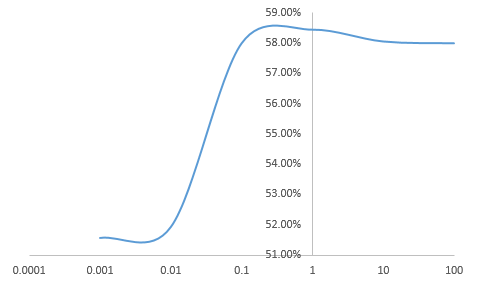
\includegraphics[width=8.0cm]{svmcurve.PNG} 
\newline
\caption{Result of SVM with Different C}
\label{fig:svmcurve} 
\end{figure}


We adopt support vector machine with 10-fold cross-validation for this problem. Correctly Classified Instances are 9445 which takes 58.5528 \%. And Incorrectly Classified Instances are 6694 which takes 41.4772 \%. 


\subsection{Results from Other Models}
We also applied other models to the problem.
 The results are shown in Table~\ref{table:others}

\begin{table}
\begin{center}
\begin{tabular}{|c|c|}
\hline
Model & Accuracy Rate \\ \hline
Decision Tree & 58.05\% \\ \hline
Natural Network & 54.98\% \\ \hline
Support Vector Machine & 58.55\% \\ \hline
Naive Bayes & 56.07\% \\ \hline
Adaboost & 55.35\% \\ \hline
\end{tabular}
\caption{Results from Other Models}
\label{table:others}
\end{center}
\end{table}

In adaboost method, we used decision tree as a classifier of it. However, we didn't find an obvious relationship between accuracy rate and the number of weak classifiers. We believe the result could be improved with more testing.

\subsection{K-nearest neighbor}

We adopt K-nearest neighbor as we discussed in the design part. Correctly Classified Instances are 8576 which takes 75.1038 \%. And Incorrectly Classified Instances are 6198 which takes 24.8962 \%. The accuracy by class and confusion matrix can be seen in Table~\ref{table:knnaccuracy} and Table~\ref{table:knnconfusionmatrix}.

\begin{table}
\begin{center}
\begin{tabular}{|c|c|c|c|}
\hline
Class & Precision & Recall & F-score \\ \hline
win & 0.702 & 0.770 & 0.734 \\ \hline
lose & 0.799 & 0.736 & 0.766 \\ \hline
\end{tabular}
\caption{Detailed Accuracy by Class}
\label{table:knnaccuracy}
\end{center}
\end{table}

\begin{table}
\begin{center}
\begin{tabular}{|c|c|c|}
\hline
a & b & \\ \hline
5546 & 1659 & a = win \\ \hline
2359 & 6575 & b = lose \\ \hline
\end{tabular}
\caption{Confusion Matrix of Decision Tree}
\label{table:knnconfusionmatrix}
\end{center}
\end{table}

From this result, we know that this modified method improved accuracy rate.

First, query the heroes with frequency in the matches;
Find first 30 heroes that appears most to set as clustering center k
use k means clustering to partition the n observations into k (≤ n) sets
